%----------------------------------------------
%LaTeX Document written by Max Stillwell
%Don't forget to compile twice! TOC will
%be missing if you don't.
%----------------------------------------------
\documentclass[12pt]{report}
\usepackage{parskip}
\usepackage[top=1in,right=1in,left=1in,bottom=1in]{geometry}
\usepackage{graphicx}
\usepackage{url}
\usepackage{fancyhdr}
\usepackage{multirow}
\usepackage{hyperref}
\hypersetup{bookmarks=true, unicode=false, pdftoolbar=true, pdfmenubar=true, pdfstartview={FitV}, pdftitle={SYSTEMS AND SOFTWARE REQUIREMENTS SPECIFICATION (SSRS) FOR Groups in a University Setting}, pdfauthor={UI CS 383 gusPY Group}, pdfkeywords={gus} {CS} {UI} {Idaho} {University}, pdfnewwindow=true, colorlinks=true, linkcolor=blue, citecolor=green, filecolor=magenta, urlcolor=blue}

\fancyhf{}
\headheight 14.49998pt
\pagestyle{fancy}
\rhead{NOT FOR RELEASE}
\lfoot{gus SSRS}
\cfoot{PAGE}
\rfoot{\thepage}

\setlength{\parskip}{0pt}
\setlength{\parindent}{0.6cm}

\setcounter{tocdepth}{4}
\setcounter{secnumdepth}{4}

\begin{document}
\pagenumbering{alph}
\pdfbookmark[1]{TITLE}{titlepage}
\begin{titlepage}
 \textbf{
  {\centering \small
   SYSTEMS AND SOFTWARE REQUIREMENTS SPECIFICATION (SSRS) FOR \\[0.5cm]
   Groups in a University Setting \\[0.5cm]
   \includegraphics{gus_Logo} \\[1cm]
   Version 0.9 \\
   \today \\[1cm]
   Prepared for: \\
   Dr. Clinton Jeffery \\[1cm]
   Prepared by: \\
   gusPY \\
   University of Idaho \\
   Moscow, ID 83844-1010 \\
  }
 }
\vfill
\end{titlepage}
\newpage

\pagenumbering{roman}
\setcounter{page}{1}
\pdfbookmark[1]{RECORD OF CHANGES}{recordofchanges}
{\centering 
 gus SSRS \\[0.3cm] 
 RECORD OF CHANGES \\[0.5cm]
 \begin{tabular}{| p{1.5cm} | p{1.5cm} | p{3cm} | p{0.5cm} | p{4cm} | p{2.2cm} | p{2cm} |}
  \hline
  Change Number & Date Completed & Location of Change (e.g. page or figure \#) & A M D & Brief Description of Change & Approved by (initials) & Date Approved \\ \hline
  1 & 12/7/10 & Section 3.2 & M & Updated Use Cases & MFS & 12/7/10 \\ \hline
  2 & 12/8/10 & Section 1.4 & M & Updated Definitions, Acronyms, and Abbreviations & MFS & 12/8/10 \\ \hline  
  3 & 12/8/10 & All Sections & M & Links, GUS to gus & MFS & 12/8/10 \\ \hline 
  & & & & & &  \\ \hline  
  & & & & & &  \\ \hline  
  & & & & & &  \\ \hline  
  & & & & & &  \\ \hline
  & & & & & &  \\ \hline
  & & & & & &  \\ \hline
  & & & & & &  \\ \hline
  & & & & & &  \\ \hline
  & & & & & &  \\ \hline
  & & & & & &  \\ \hline
  & & & & & &  \\ \hline
  & & & & & &  \\ \hline
  & & & & & &  \\ \hline
  & & & & & &  \\ \hline
  & & & & & &  \\ \hline
  & & & & & &  \\ \hline
  & & & & & &  \\ \hline
 \end{tabular}
}
\newline
A - ADDED M - MODIFIED D - DELETED
\newpage


\pdfbookmark[1]{CONTENTS}{tableofcontents}
\tableofcontents
\newpage

\pagenumbering{arabic}
\setcounter{page}{1}
\renewcommand*\thesection{\arabic{section}}
\section{INTRODUCTION}
 \subsection{IDENTIFICATION}
  The software system being considered for development is referred to as \htmlref{Groups in a University Setting}{Groups on a University Setting} or \htmlref{gus}{gus}. The specifications for the system are being developed by the team itself. The ultimate customer, or end-user, of the system will be universities or similar institutions including but not limited to the University of Idaho. This is a new project effort, so the version under development is version 1.0.
 \subsection{PURPOSE}
  The purpose of the system under development is to provide a tool for the easy administration and control of university-style groups including but not limited to clubs and sports teams. While the system will be used by university personnel, this document is intended to be read and understood by UICS software designers and coders.
 \subsection{SCOPE}
  \begin{enumerate}
    \item Simplifying tasks down to things only leaders of groups will be required to do, such as:
    \begin{enumerate}
     \item Sending notifications to group members (email)
     \item Sending information (files) to group members via email or download link
     \item Managing a group-wide calendar of events
     \item Automatically generating:
      \begin{enumerate}
       \item Contact information (contact sheets, phone directories)
       \item Website with updated contact, group, event, and customized information
       \item Organization charts
       \item Graphical relationships between groups
       \item Fees, dues, and expenses notifications
      \end{enumerate}
    \end{enumerate}
   \item Consolidating information for members and potential members of groups:
    \begin{enumerate}
     \item Common location of group information
     \item Searching existing groups
     \item Tying together existing groups (even suggesting similar groups)
     \item Personalized emails regarding changes/updates
     \item Outstanding expenses or reimbursements
     \item Reliable (i.e., automatically updated):
      \begin{enumerate}
       \item Group contact information
       \item Group event information
      \end{enumerate}
    \end{enumerate}
  \end{enumerate}
 \subsection{DEFINITIONS, ACRONYMS, AND ABBREVIATIONS}
  \begin{center}
   \begin{tabular}{| p{4cm} | p{12cm} |}
     \hline
      \textbf{Term or Acronym} & \textbf{Definition} \\ \hline
      \label{Administrator}Administrator & A user who has administrative privileges for a Group or Groups. \\ \hline
      \label{Admin}Admin & \htmlref{Administrator}{Administrator} \\ \hline
      Alpha test & Limited release(s) to selected, outside testers. \\ \hline
      Beta test & Limited release(s) to cooperating customers wanting early access to developing systems. \\ \hline
      DFD & Data Flow Diagram. \\ \hline
      Final test & aka, Acceptance test, release of full functionality to customer for approval. \\ \hline
      \label{Group}Group & A collection of Groups and/or Members that has an assigned \htmlref{Owner}{Owner}. \\ \hline
      \label{gus}gus & Groups in a University Setting \\ \hline
      \label{gusPY}gusPY & Groups in a University Setting - Python Implemnetation. \\ \hline
      \label{Member}Member & A user who has an account and is part of a \htmlref{Group}{Group}. \\ \hline
      \label{Non-Member}Non-Member & A user who does not have an account and is not a \htmlref{Member}{Member} of any \htmlref{Group}{Group}. \\ \hline
      \label{Owner}Owner & A user who is an \htmlref{Owner}{Owner} of a \htmlref{Group}{Group}. \\ \hline
      \label{Pseudo-Member}Pseudo-Member & A user who does not have an account of their own, but is still considered to be part of a \htmlref{Group}{Group}. \\ \hline
      \label{SDD}SDD & Software Design Document, aka SDS, Software Design Specification. \\ \hline
      \label{SRS}SRS & Software Requirements Specification. \\ \hline
      \label{SSRS}SSRS & System and Software Requirements Specification. \\ \hline
   \end{tabular}
  \end{center}
 \subsection{REFERENCES}
  gus proposal: {\small \url{http://www2.cs.uidaho.edu/~jeffery/courses/383/hw1/solomon_kopriva.pdf}}
 \newpage
 \subsection{OVERVIEW AND RESTRICTIONS}
  This document is for limited release only to UI CS personnel working on the project. \\[0.4cm]
  \indent Section 2 of this document describes the system under development from a holistic point of view. Functions, characteristics, constraints, assumptions, dependencies, and overall requirements are defined from the system-level perspective. \\[0.4cm]
  \indent Section 3 of this document describes the specific requirements of the system being developed. Interfaces, features, and specific requirements are enumerated and described to a degree sufficient for a knowledgeable designer or coder to begin crafting and architectural solution to the proposed system. \\[0.4cm]
  \indent Section 4 provides the requirements traceability information for the project. Each feature of the system is indexed by the \htmlref{SSRS}{SSRS} requirement number and linked to its \htmlref{SDD}{SDD} and test references.
  %\indent Sections 5 and up are appendices including original information and communications used to create this document.

\newpage
\section{OVERALL DESCRIPTION}
 \subsection{PRODUCT PERSPECTIVE}
  \htmlref{Gus}{gus} is an independent software system, as it does not directly integrate with a larger system. However, \htmlref{gus}{gus} does draw data from external sources, such as personal information databases, and needs to be integrated with a web server in order to be readily accessible.
 \subsection{PRODUCT FUNCTIONS}
  \htmlref{Gus}{gus} is a system for managing groups of people, specifically in a university setting. It tries to maintain a balance between generality and domain-specific paradigms. While \htmlref{gus}{gus} could be used to manage groups of people in any setting, it contains a set of defaults and tunings specific to a university.\newline
  \indent Managing people includes sending messages and files to groups of people, automatically generating human and machine-readable information such as contact sheets, organization charts, and calendars, helping people find groups they would like to be a part of, automating fee and expense notifications, and consolidating information about groups in an automatically-generated web site.
 \subsection{USER CHARACTERISTICS}
  \htmlref{Gus}{gus} should be easy for any user to understand with a brief explanation and intuitive enough for an uninitiated user to figure out by looking through the options. Basic computer use skills and a simple conceptual explanation should be enough for every day usage.
 \subsection{CONSTRAINTS}
  \htmlref{Gus}{gus} needs to be able to interface with any data source it needs information from, which could prove to be personnel databases and authentication servers. It must support multiple user connections at the same time. It should be reliable with little maintenance, and be secure enough to be accessible by legitimate from the Internet proper.
 \subsection{ASSUMPTIONS AND DEPENDICIES}
  It is assumed that the \htmlref{gus}{gus} server will run on a Unix-like system, but it may be necessary to port it to other operating systems. Enough bandwidth to support the maximum estimated concurrent users must be provided.
 \subsection{SYSTEM LEVEL (NON-FUNCTIONAL) REQUIREMENTS}
  \subsubsection{Site Dependencies}
   \htmlref{Gus}{gus} will need a Unix-like server to run on, with sufficient bandwidth and processing power to serve the estimated number of concurrent users. It will require a database in which to store its data.
  \subsubsection{Safety, Security and Privacy Requirements}
   Apart from standard security that servers connected to the Internet require, \htmlref{gus}{gus} will need a secure authentication system. Secure access and authentication is important, but most of the security requirements are related to access, and will be handled by the hierarchy of people in charge. \htmlref{gus}{gus} cannot prevent a group leader from distributing contact information, but it can provide a framework for disallowing unauthorized access to the information.
  \subsubsection{Performance Requirements}
   \htmlref{Gus}{gus} must be able to handle at least thirty-five simultaneous users with all transactions visible to the user within one second (given ideal network speeds).
  \subsubsection{System and Software Quality}
   \htmlref{Gus}{gus} must perform all required functions, behave consistently and correctly, be easily corrected, always running, generalized enough to be easily adaptable, test-driven, and easy to use.
  \subsubsection{Packaging and Delivery Requirements}
   The executable system and all associated documentation (i.e., \htmlref{SSRS}{SSRS}, \htmlref{SDD}{SDD}, code listing, test plan (data and results), and user manual) will be delivered to the customer via internet download. The final, edited version of the above documents will accompany the final, accepted version of the executable system.
  \subsubsection{Personnel-related Requirements}
   The system under development has no special personnel-related characteristics.
  \subsubsection{Training-related Requirements}
   No training materials or expectations are tied to this project other than user manual that will accompany the software.
  \subsubsection{Logistics-related Requirements}
   A server will be required to maintain the software system. The user will be required to have a reasonable internet connection.

\newpage
\section{SPECIFIC REQUIREMENTS}
 \subsection{EXTERNAL INTERFACE REQUIREMENTS}
  \subsubsection{Hardware Interfaces}
   The system will require a server that can run Python 2.7, Django, and has secure networking capabilities.
  \subsubsection{Software Interfaces}
   The system will require Python 2.7 \& Django.
  \subsubsection{User Interfaces}
   The system will require a compatiable web browser and 3 different user interfaces for \htmlref{Member}{Members}, \htmlref{Owner}{Owners}, and \htmlref{Administrator}{Administrators}.
   \newpage
   {\centering \textbf{External Interface Requirements} \\[0.1cm]
   \begin{tabular}{| p{2cm} | p{2cm} | p{5cm} | p{2cm} | p{2.8cm} | p{1.6cm} |}
    \hline
     \textbf{Name} & \textbf{Source / Destination} & \textbf{Description} & \textbf{Type / Range} & \textbf{Dependencies} & \textbf{Formats} \\ \hline
     HTTP Server & Dedicated Server or VPS / Client & This Device is responsible for serving HTML content (and other content) to clients. Preferably Apache2. & All & Requires a server capable machine. & N/A \\ \hline
     VPS or Dedicated Server & N/A & A VPS or a Dedicated Server, preferably running a preconfigured Linux distribution such as Fedora or Ubuntu. & All & Electricity, high-speed internet connection. & N/A \\ \hline
   \end{tabular}\\[0.1cm]}
   {\centering \textbf{Software Interfaces} \\[0.1cm]
   \begin{tabular}{| p{2cm} | p{2cm} | p{5cm} | p{2cm} | p{2.8cm} | p{1.6cm} |}
    \hline
     \textbf{Name} & \textbf{Source / Destination} & \textbf{Description} & \textbf{Type / Range} & \textbf{Dependencies} & \textbf{Formats} \\ \hline
     SQL Server & Dedicated Server or VPS & Works in conjunction with HTTP server to provide data. & All & Requires a server-capable machine. & N/A \\ \hline
     Python 2.7 \& Django & Provides computational power so tasks that serve HTML content can be completed. & All & Requires a server-capable of running Python 2.7 & Django. & N/A \\ \hline
   \end{tabular}\\[0.1cm]}
   {\centering \textbf{User Interfaces} \\[0.1cm]
   \begin{tabular}{| p{2cm} | p{2cm} | p{5cm} | p{2cm} | p{2.8cm} | p{1.6cm} |}
    \hline
     \textbf{Name} & \textbf{Source / Destination} & \textbf{Description} & \textbf{Type / Range} & \textbf{Dependencies} & \textbf{Formats} \\ \hline
     Website & HTTP Server / Client & Allows users to interact with the service. & All & HTTP Server & Web \\ \hline
   \end{tabular}\\[0.1cm]}
   {\centering \textbf{Other Communication Interfaces} \\[0.1cm]
   \begin{tabular}{| p{2cm} | p{2cm} | p{5cm} | p{2cm} | p{2.8cm} | p{1.6cm} |}
    \hline
     \textbf{Name} & \textbf{Source / Destination} & \textbf{Description} & \textbf{Type / Range} & \textbf{Dependencies} & \textbf{Formats} \\ \hline
     N/A & N/A & N/A & N/A & N/A & N/A \\ \hline
   \end{tabular}\\[0.1cm]}
 \subsection{SYSTEM FEATURES}
  \subsubsection{Use Case Diagrams}
    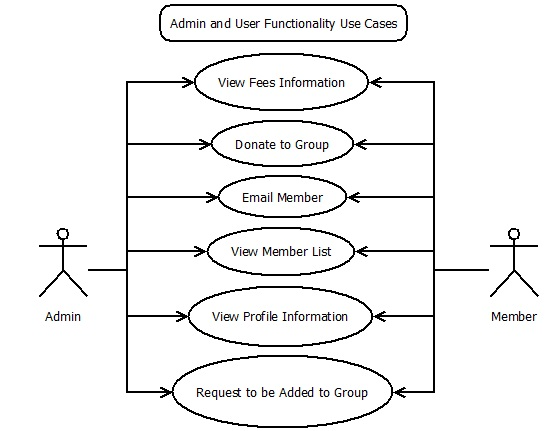
\includegraphics{AdminUser_UseCase} \\[1.0cm]
    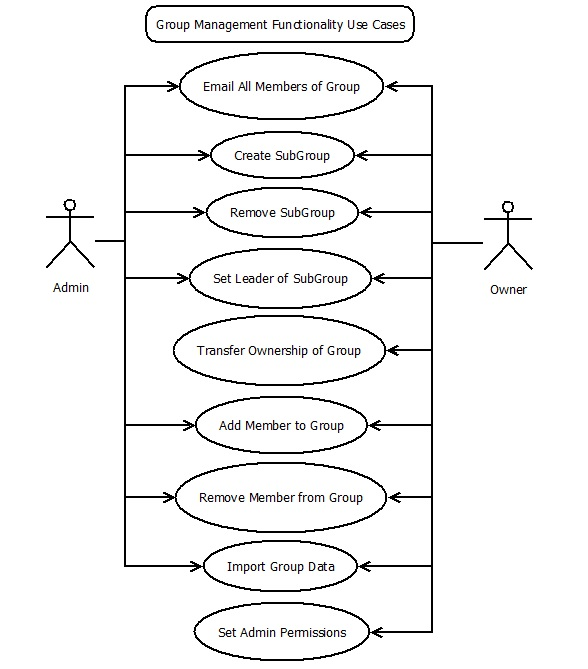
\includegraphics{GroupManagement_UseCase} \\[1.0cm]
    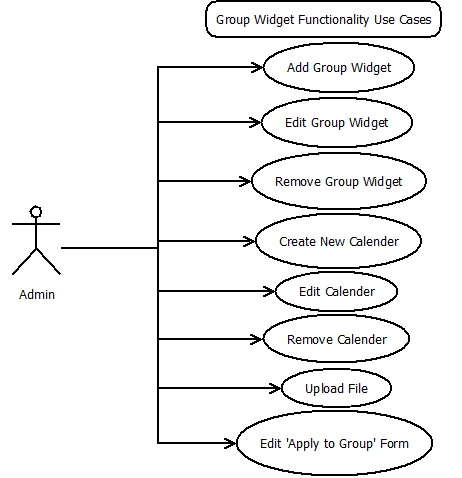
\includegraphics{GroupWidget_UseCase} \\[1.0cm]
  \subsubsection{System Feature 1: View Fees Information}
    \begin{tabular}{ | p{16cm} | }
     \hline
      \textbf{Use Case Description} \\ \hline
       \textbf{Actors:} \htmlref{Member}{Member}, \htmlref{Admin}{Admin}\\ 
       \textbf{Goals:} To allow \htmlref{Member}{Members} to view if they have paid their fees, as well as allow \htmlref{Administrator}{Administrators} to view the list of who has and hasn't paid their fees.\\
       \textbf{Preconditions:} To view the list of paid fees User must be logged in as an \htmlref{Admin}{Admin}. For a \htmlref{Member}{Member} to view if they have paid their fees they must be logged in as a \htmlref{Member}{Member}.\\
       \textbf{Summary} \\
       This allows the tracking of fee payment. It does not in any way facilitate the transfer of money, it will only allow for the \htmlref{Administrator}{Administrators} to keep track of who has paid.\\ \\
       \textbf{Steps:}
       \begin{enumerate}
        \item User clicks the ``Profile'' link on the \htmlref{gus}{gus} pages.
        \item Inside the profile page there will be a section titled ``Fees'' where there will be a marking of paid or not.
       \end{enumerate} \\ \hline
    \end{tabular}

   \subsubsection{System Feature 2: Donate to Group}
    \begin{tabular}{ | p{16cm} | }
     \hline
      \textbf{Use Case Description} \\ \hline
       \textbf{Actors:} \htmlref{Member}{Member}, \htmlref{Admin}{Admin}, \htmlref{Non-Member}{Non-Member}, \htmlref{Pseudo-Member}{Pseudo-Member}\\ 
       \textbf{Goals:} To allow \htmlref{Member}{Members} and \htmlref{Non-Member}{Non-Members} to donate money to the \htmlref{Group}{Group} for various activities.\\
       \textbf{Preconditions:} User must be viewing a specific \htmlref{Group}{Group} page, which has enabled Donations.\\
      \textbf{Summary} \\
       This will allow \htmlref{Group}{Groups} to enable a PayPal or similar account which can be donated to specifically for the \htmlref{Group}{Group}.\\ \\
      \textbf{Steps:}
       \begin{enumerate}
        \item User clicks the ``Donate'' button on the main page of a \htmlref{Group}{Group}.
        \item Follow the steps for the selected type of donation.
       \end{enumerate} \\
      \textbf{Alternatives:} \\
      \begin{enumerate}
       \item User clicks ``Cancel'' in Steps 2.
      \end{enumerate} \\ \hline
    \end{tabular}

   \subsubsection{System Feature 3: Email Member}
    \begin{tabular}{ | p{16cm} | }
     \hline
      \textbf{Use Case Description} \\ \hline
       \textbf{Actors:} \htmlref{Member}{Member}, \htmlref{Admin}{Admin}\\ 
       \textbf{Goals:} To allow \htmlref{Member}{Members} of a \htmlref{Group}{Group} to communicate without adding every person in every group to their email contacts.\\
       \textbf{Preconditions:} Must be logged in as either a \htmlref{Member}{Member} or \htmlref{Admin}{Admin}, and attempting to send an email to a registered \htmlref{Member}{Member}.\\
      \textbf{Summary} \\
       Will send an email to the registered email account of another User.\\ \\
      \textbf{Steps:}
       \begin{enumerate}
        \item Select ``View Members'' from a \htmlref{Group}{Group's} main page.
        \item Select ``View Profile'' from a specific \htmlref{Member}{Members} listing.
        \item Select ``Email Member''.
        \item Write Email.
        \item Click ``Submit''.
       \end{enumerate} \\
      \textbf{Alternatives:} \\
      \begin{enumerate}
       \item Select the ``Mail'' icon in Step 2, skip to Step 4.
      \end{enumerate} \\ \hline
    \end{tabular}

   \subsubsection{System Feature 4: View Member List}
    \begin{tabular}{ | p{16cm} | }
     \hline
      \textbf{Use Case Description} \\ \hline
       \textbf{Actors:} \htmlref{Member}{Member}, \htmlref{Admin}{Admin}\\ 
       \textbf{Goals:} To allow \htmlref{Member}{Members}, and \htmlref{Administrator}{Administrators} of a \htmlref{Group}{Group} to view the list of other \htmlref{Member}{Members} in the \htmlref{Group}{Group}.\\
       \textbf{Preconditions:} Must be logged in as either a \htmlref{Member}{Member} or \htmlref{Admin}{Admin} of the \htmlref{Group}{Group}.\\
      \textbf{Summary} \\
       \htmlref{Member}{Members} will have privacy options to prevent their listing from showing up to everyone, except \htmlref{Administrator}{Administrators}.\\ \\
      \textbf{Steps:}
       \begin{enumerate}
        \item Select ``View Members'' from a \htmlref{Group}{Group's} main page.
       \end{enumerate} \\ \hline
    \end{tabular}

   \subsubsection{System Feature 5: View Profile Information}
    \begin{tabular}{ | p{16cm} | }
     \hline
      \textbf{Use Case Description} \\ \hline
       \textbf{Actors:} \htmlref{Member}{Member}, \htmlref{Admin}{Admin}\\ 
       \textbf{Goals:} To allow \htmlref{Member}{Members} and \htmlref{Administrator}{Administrators} of a \htmlref{Group}{Group} to view the list of other \htmlref{Member}{Members} in the \htmlref{Group}{Group}.\\
       \textbf{Preconditions:} Must be logged in as a \htmlref{Member}{Member} or \htmlref{Admin}{Admin} to the same \htmlref{Group}{Group} as the \htmlref{Member}{Member} to be viewed.\\
      \textbf{Summary} \\
       \htmlref{Member}{Members} will have privacy options to prevent their information from showing up to everyone, except \htmlref{Administrator}{Administrators}.\\ \\
      \textbf{Steps:}
       \begin{enumerate}
        \item Select ``View Members'' from a \htmlref{Group}{Group} main page.
        \item Select ``View Profile'' from a specific \htmlref{Member}{Member's} listing.
       \end{enumerate} \\ \hline
    \end{tabular}

   \subsubsection{System Feature 6: Request to be Added to Group}
    \begin{tabular}{ | p{16cm} | }
     \hline
      \textbf{Use Case Description} \\ \hline
       \textbf{Actors:} \htmlref{Member}{Member}, \htmlref{Non-Member}{Non-Member}, \htmlref{Pseudo-Member}{Pseudo-Member}\\
       \textbf{Goals:} To allow \htmlref{Non-Member}{Non-Members} to request addition to a \htmlref{Group}{Group}.\\
       \textbf{Preconditions:} Must not be a \htmlref{Member}{Member} of the selected \htmlref{Group}{Group}, viewing the desired \htmlref{Group}{Group's} main page.\\
      \textbf{Summary} \\
       Allows \htmlref{Non-Member}{Non-Members} of a \htmlref{Group}{Group} to be added so they can view the various Widgets that \htmlref{Group}{Group} has added, and receive notifications.\\ \\
      \textbf{Steps:}
       \begin{enumerate}
        \item Click the ``Apply to Group'' button.
        \item Fill out the form required by the \htmlref{Owner}{Owner} of the \htmlref{Group}{Group}.
        \item Click ``Submit''.
       \end{enumerate} \\
      \textbf{Alternatives:} \\
      \begin{enumerate}
       \item User clicks ``Cancel'' in Step 2.
      \end{enumerate} \\ \hline
    \end{tabular}

   \subsubsection{System Feature 7: Email All Members of Group}
    \begin{tabular}{ | p{16cm} | }
     \hline
      \textbf{Use Case Description} \\ \hline
       \textbf{Actors:} \htmlref{Owner}{Owner}, \htmlref{Admin}{Admin}\\ 
       \textbf{Goals:} To allow \htmlref{Administrator}{Administrators} and \htmlref{Owner}{Owners} to send out \htmlref{Group}{Group} email.\\
       \textbf{Preconditions:} Must be logged in as \htmlref{Admin}{Admin} or \htmlref{Owner}{Owner}.\\
      \textbf{Summary} \\
       Will send out an email to everyone in the \htmlref{Group}{Group}, including the \htmlref{Administrator}{Administrators} and \htmlref{Owner}{Owners}.\\ \\
      \textbf{Steps:}
       \begin{enumerate}
        \item Select ``View Group Members'' from the main page.
        \item Click ``Email Group''.
        \item Write the Email.
        \item Click ``Send''.
       \end{enumerate} \\
      \textbf{Alternatives:} \\
      \begin{enumerate}
       \item User clicks ``Cancel'' in Step 3.
      \end{enumerate} \\ \hline
    \end{tabular}

   \subsubsection{System Feature 8: Create Sub-Group}
    \begin{tabular}{ | p{16cm} | }
     \hline
      \textbf{Use Case Description} \\ \hline
       \textbf{Actors:} \htmlref{Owner}{Owner}, \htmlref{Admin}{Admin}\\ 
       \textbf{Goals:} To allow a \htmlref{Group}{Group} to organize their \htmlref{Member}{Members} into \htmlref{Group}{Groups}.\\
       \textbf{Preconditions:} Must be logged in as \htmlref{Admin}{Admin} or \htmlref{Owner}{Owner}.\\
      \textbf{Summary} \\
       Will create a new \htmlref{Group}{Group}, with the \htmlref{Owner}{Owner} being the same as the Super-Group.\\ \\
      \textbf{Steps:}
       \begin{enumerate}
        \item Enter Admin Mode by clicking the ``Admin'' link.
        \item Go to the ``Group Management'' tab.
        \item Click ``Create Sub-Group''.
        \item Fill out information required.
        \item Click ``Submit''.
       \end{enumerate} \\
      \textbf{Alternatives:} \\
      \begin{enumerate}
       \item User clicks ``Cancel'' in Step 4.
      \end{enumerate} \\ \hline
    \end{tabular}

   \subsubsection{System Feature 9: Remove Sub-Group}
    \begin{tabular}{ | p{16cm} | }
     \hline
      \textbf{Use Case Description} \\ \hline
       \textbf{Actors:} \htmlref{Owner}{Owner}, \htmlref{Admin}{Admin}\\ 
       \textbf{Goals:} To allow \htmlref{Owner}{Owners} and \htmlref{Administrator}{Administrators} to remove un-needed Sub-Groups.\\
       \textbf{Preconditions:} Logged in as \htmlref{Admin}{Admin} or \htmlref{Owner}{Owner}, and the given Sub-Group must be a Sub-Group of their \htmlref{Group}{Group}.\\
      \textbf{Summary} \\
       Will remove the given Sub-Group.\\ \\
      \textbf{Steps:}
       \begin{enumerate}
        \item Enter Admin Mode by clicking the ``Admin'' link.
        \item Go to the ``Group Management'' tab.
        \item Click ``Delete'' next to the desired Sub-Group.
        \item Click ``Ok''.
       \end{enumerate} \\
      \textbf{Alternatives:} \\
      \begin{enumerate}
       \item User clicks ``Cancel'' in Step 3.
      \end{enumerate} \\ \hline
    \end{tabular}

   \subsubsection{System Feature 10: Set Leader of Sub-Group}
    \begin{tabular}{ | p{16cm} | }
     \hline
      \textbf{Use Case Description} \\ \hline
       \textbf{Actors:} \htmlref{Owner}{Owner}, \htmlref{Admin}{Admin}\\ 
       \textbf{Goals:} To allow \htmlref{Owner}{Owners} and \htmlref{Administrator}{Administrators} to set a different \htmlref{Owner}{Owner} of the Sub-Groups.\\
       \textbf{Preconditions:} Logged in as \htmlref{Admin}{Admin} or \htmlref{Owner}{Owner}, and the given Sub-Group must be a Sub-Group of their \htmlref{Group}{Group}.\\
      \textbf{Summary} \\
       Will make the \htmlref{Owner}{Owner} of the desired Sub-Group a different User.\\ \\
      \textbf{Steps:}
       \begin{enumerate}
        \item Enter Admin Mode by clicking the ``Admin'' link.
        \item Go to the ``Group Management'' tab.
        \item Click ``Change Owner'' next to the desired Group.
        \item Choose new Owner.
        \item Click ``Ok''.
       \end{enumerate} \\
      \textbf{Alternatives:} \\
      \begin{enumerate}
       \item User clicks ``Cancel'' in Step 4.
      \end{enumerate} \\ \hline
    \end{tabular}

   \subsubsection{System Feature 11: Transfer Ownership of Group}
    \begin{tabular}{ | p{16cm} | }
     \hline
      \textbf{Use Case Description} \\ \hline
       \textbf{Actors:} \htmlref{Owner}{Owner}\\ 
       \textbf{Goals:} Allow an \htmlref{Owner}{Owner} to give ownership of a \htmlref{Group}{Group} to a different \htmlref{Member}{Member}.\\
       \textbf{Preconditions:} Must be logged in as \htmlref{Owner}{Owner}, and there must be at least 1 other \htmlref{Member}{Member} in the \htmlref{Group}{Group}.\\
      \textbf{Summary} \\
       Will make the \htmlref{Owner}{Owner} of the current \htmlref{Group}{Group} a different \htmlref{Member}{Member}.\\ \\
      \textbf{Steps:}
       \begin{enumerate}
        \item Enter Admin Mode by clicking the ``Admin'' link.
        \item Go to the ``Group Management'' tab.
        \item Click ``Change Owner''.
        \item Choose new Owner.
        \item Click ``Ok''.
       \end{enumerate} \\
      \textbf{Alternatives:} \\
      \begin{enumerate}
       \item User clicks ``Cancel'' in Step 4.
      \end{enumerate} \\ \hline
    \end{tabular}

   \subsubsection{System Feature 12: Add Member to Group}
    \begin{tabular}{ | p{16cm} | }
     \hline
      \textbf{Use Case Description} \\ \hline
       \textbf{Actors:} \htmlref{Owner}{Owner}, \htmlref{Admin}{Admin}\\ 
       \textbf{Goals:} To allow the addition of new \htmlref{Member}{Members} to a \htmlref{Group}{Group}.\\
       \textbf{Preconditions:} Must be logged in as \htmlref{Admin}{Admin} or \htmlref{Owner}{Owner}, and new \htmlref{Member}{Member} must not already be a \htmlref{Member}{Member}.\\
      \textbf{Summary} \\
       Will add a new \htmlref{Member}{Member} to the \htmlref{Group}{Group}.\\ \\
      \textbf{Steps:}
       \begin{enumerate}
        \item Enter Admin Mode by clicking the ``Admin'' link.
        \item Go to the ``Group Management'' tab.
        \item Click ``Add Member''.
        \item Fill out the required information.
        \item Click ``Submit''.
       \end{enumerate} \\
      \textbf{Alternatives:} \\
      \begin{enumerate}
       \item User clicks ``Cancel'' in Step 4.
      \end{enumerate} \\ \hline
    \end{tabular}

   \subsubsection{System Feature 13: Remove Member from Group}
    \begin{tabular}{ | p{16cm} | }
     \hline
      \textbf{Use Case Description} \\ \hline
       \textbf{Actors:} \htmlref{Owner}{Owner}, \htmlref{Admin}{Admin}\\ 
       \textbf{Goals:} To allow \htmlref{Owner}{Owners} and \htmlref{Admin}{Admin} to remove unwanted or absent \htmlref{Member}{Members} of a \htmlref{Group}{Group}.\\
       \textbf{Preconditions:} Must be logged in as \htmlref{Admin}{Admin} or \htmlref{Owner}{Owner} and desired \htmlref{Member}{Member} must be a \htmlref{Member}{Member} of the \htmlref{Group}{Group}.\\
      \textbf{Summary} \\
       Will remove the desired \htmlref{Member}{Member}, taking away any permission they had.\\ \\
      \textbf{Steps:}
       \begin{enumerate}
        \item Enter Admin Mode by clicking the ``Admin'' link.
        \item Go to the ``Group Management'' tab.
        \item Select ``Manage Members''.
        \item Select the Member to manage.
        \item Click the ``Remove From Group'' button.
        \item Click ``Ok''.
       \end{enumerate} \\
      \textbf{Alternatives:} \\
      \begin{enumerate}
       \item User clicks ``Cancel'' in Step 3 or 5.
      \end{enumerate} \\ \hline
    \end{tabular}

   \subsubsection{System Feature 14: Import Group Data}
    \begin{tabular}{ | p{16cm} | }
     \hline
      \textbf{Use Case Description} \\ \hline
       \textbf{Actors:} \htmlref{Owner}{Owner}, \htmlref{Admin}{Admin}\\ 
       \textbf{Goals:} To allow \htmlref{Owner}{Owners} and \htmlref{Administrator}{Administrators} to import \htmlref{gus}{gus} \htmlref{Group}{Group} data from an external source such as Excel.\\
       \textbf{Preconditions:} Must be logged in as \htmlref{Owner}{Owner} or \htmlref{Admin}{Admin}.\\
      \textbf{Summary} \\
       Will first check the list of Users against the current list of \htmlref{Member}{Members} in the \htmlref{Group}{Group}, then it will add all of the \htmlref{Non-Member}{Non-Members}.\\ \\
      \textbf{Steps:}
       \begin{enumerate}
        \item Enter Admin Mode by clicking the ``Admin'' link.
        \item Go to the ``Group Management'' tab.
        \item Select ``Import Group Data''.
        \item Browse for the file on the local machine.
        \item Click ``Import''.
       \end{enumerate} \\
      \textbf{Alternatives:} \\
      \begin{enumerate}
       \item User clicks ``Cancel'' in Step 4.
      \end{enumerate} \\ \hline
    \end{tabular}

   \subsubsection{System Feature 15: Set Admin Permissions}
    \begin{tabular}{ | p{16cm} | }
     \hline
      \textbf{Use Case Description} \\ \hline
       \textbf{Actors:} \htmlref{Owner}{Owner}\\ 
       \textbf{Goals:} To allow \htmlref{Owner}{Owners} to delegate most of the tasks of administering a \htmlref{Group}{Group}.\\
       \textbf{Preconditions:} Must be logged in as \htmlref{Owner}{Owner}, and desired \htmlref{Member}{Members} must be \htmlref{Member}{Members} of current \htmlref{Group}{Group}.\\
      \textbf{Summary} \\
       Will set varying levels of permissions to different \htmlref{Member}{Members} of the \htmlref{Group}{Group}.\\ \\
      \textbf{Steps:}
       \begin{enumerate}
        \item Enter Admin Mode by clicking the ``Admin'' link.
        \item Go to the ``Group Management'' tab.
        \item Select ``Manage Members''.
        \item Select the Member to manage.
        \item Select ``Change Permissions''.
        \item Fill out the required information.
        \item Click ``Save''.
       \end{enumerate} \\
      \textbf{Alternatives:} \\
      \begin{enumerate}
       \item User clicks ``Cancel'' in Step 4 or 6.
      \end{enumerate} \\ \hline
    \end{tabular}

   \subsubsection{System Feature 16: Add Group Widget}
    \begin{tabular}{ | p{16cm} | }
     \hline
      \textbf{Use Case Description} \\ \hline
       \textbf{Actors:} \htmlref{Admin}{Admin}\\ 
       \textbf{Goals:} To allow \htmlref{Administrator}{Administrators} to add the many different components available in \htmlref{gus}{gus}.\\
       \textbf{Preconditions:} Be logged in as an \htmlref{Admin}{Admin}.\\
      \textbf{Summary} \\
        There are many different components in \htmlref{gus}{gus}, and they will all have the same basic Use Cases, Add/Edit/Remove, allowing \htmlref{Administrator}{Administrators} to add new Widgets, edit existing Widgets, and remove Widgets.\\ \\
      \textbf{Steps:}
       \begin{enumerate}
        \item Enter Admin Mode by clicking the ``Admin'' link on a \htmlref{gus}{gus} \htmlref{Group}{Group} Page.
        \item Click the ``Add/Edit/Remove Component'' tab in the \htmlref{Admin}{Admin} Panel.
        \item Click ``Add New Component''.
        \item Select a component from the list.
        \item Fill out any necessary information for the component.
        \item Click ``Add''.
       \end{enumerate} \\
      \textbf{Alternatives:} \\
      \begin{enumerate}
       \item User clicks ``Cancel'' in Step 3, 4, or 5.
      \end{enumerate} \\ \hline
    \end{tabular}

   \subsubsection{System Feature 17: Edit Group Widget}
    \begin{tabular}{ | p{16cm} | }
     \hline
      \textbf{Use Case Description} \\ \hline
       \textbf{Actors:} \htmlref{Admin}{Admin}\\ 
       \textbf{Goals:} To allow editing, specific to each widget in \htmlref{gus}{gus}.\\
       \textbf{Preconditions:} Be logged in as an \htmlref{Admin}{Admin}, and have Widgets already added to the \htmlref{Group}{Group}.\\
      \textbf{Summary} \\
        There are many different components in \htmlref{gus}{gus}, and they will all have the same basic Use Cases, Add/Edit/Remove, allowing Administrators to add new Widgets, edit existing Widgets, and remove Widgets.\\ \\
      \textbf{Steps:}
       \begin{enumerate}
        \item Enter Admin Mode by clicking the ``Admin'' link on a \htmlref{gus}{gus} \htmlref{Group}{Group} Page.
        \item Click the ``Add/Edit/Remove Component'' tab in the \htmlref{Admin}{Admin} Panel.
        \item Click on a component to enter edit mode.
        \item Make the desired changed.
        \item Click ``Save''.
       \end{enumerate} \\
      \textbf{Alternatives:} \\
      \begin{enumerate}
       \item User clicks ``Cancel'' in Step 3, 4 or 5.
      \end{enumerate} \\ \hline
    \end{tabular}

   \subsubsection{System Feature 18: Remove Group Widget}
    \begin{tabular}{ | p{16cm} | }
     \hline
      \textbf{Use Case Description} \\ \hline
       \textbf{Actors:} \htmlref{Admin}{Admin}\\ 
       \textbf{Goals:} To allow the removal of existing components.\\
       \textbf{Preconditions:} Be logged in as an \htmlref{Admin}{Admin}, and have Widgets already added to the \htmlref{Group}{Group}.\\
      \textbf{Summary} \\
        There are many different components in \htmlref{gus}{gus}, and they will all have the same basic Use Cases, Add/Edit/Remove, allowing Administrators to add new Widgets, edit existing Widgets, and remove Widgets.\\ \\
      \textbf{Steps:}
       \begin{enumerate}
        \item Enter Admin Mode by clicking the ``Admin'' link on a \htmlref{gus}{gus} \htmlref{Group}{Group} Page.
        \item Click the ``Add/Edit/Remove Component'' tab in the \htmlref{Admin}{Admin} Panel.
        \item Click on a component to enter edit mode.
        \item Click ``Remove Component''.
        \item Click ``Ok''.
       \end{enumerate} \\
      \textbf{Alternatives:} \\
      \begin{enumerate}
       \item User clicks ``Cancel'' in Step 3or 4.
      \end{enumerate} \\ \hline
    \end{tabular}

    \subsubsection{System Feature 19: Create New Calendar}
    \begin{tabular}{ | p{16cm} | }
     \hline
      \textbf{Use Case Description} \\ \hline
       \textbf{Actors:} \htmlref{Admin}{Admin}\\ 
       \textbf{Goals:} To allow \htmlref{Group}{Groups} to schedule events.\\
       \textbf{Preconditions:} Must be logged in as an \htmlref{Admin}{Admin} for the desired \htmlref{Group}{Group}.\\
      \textbf{Summary} \\
        Calendars will be able to display both time and location of events, as well as send reminder email out to specified \htmlref{Member}{Members}.\\ \\
      \textbf{Steps:}
       \begin{enumerate}
        \item Enter Admin Mode by clicking the ``Admin'' link on a \htmlref{gus}{gus} \htmlref{Group}{Group} Page.
        \item Click the ``Add/Edit/Remove Component'' tab in the \htmlref{Admin}{Admin} Panel.
        \item Click ``Add New Component''.
        \item Select ``Calendar'' from the list.
        \item Add any information required for the Calendar.
        \item Click ``Add''.
       \end{enumerate} \\
      \textbf{Alternatives:} \\
      \begin{enumerate}
       \item User clicks ``Cancel'' in Step 3, 4, or 5.
      \end{enumerate} \\ \hline
    \end{tabular}

   \subsubsection{System Feature 20: Edit Calendar}
    \begin{tabular}{ | p{16cm} | }
     \hline
      \textbf{Use Case Description} \\ \hline
       \textbf{Actors:} \htmlref{Admin}{Admin}\\ 
       \textbf{Goals:} Allow the modification of Calendars.\\
       \textbf{Preconditions:} Must be logged in as an \htmlref{Admin}{Admin}.\\
      \textbf{Summary} \\
        Events will change over time, this allows for the modification of those events, as well as creation of new events.\\
      \textbf{Steps:}
       \begin{enumerate}
        \item Enter Admin Mode by clicking the ``Admin'' link on a \htmlref{gus}{gus} \htmlref{Group}{Group} Page.
        \item Click the ``Add/Edit/Remove Component'' tab in the \htmlref{Admin}{Admin} Panel.
        \item Click on the ``Calendar'' to enter edit mode.
        \item Select the date to edit.
        \item If editing an existing event, select the event.
        \item If creating a new event click ``Add Event''.
        \item Fill out the correct information.
        \item Click ``Save''.
       \end{enumerate} \\
      \textbf{Alternatives:} \\
      \begin{enumerate}
       \item User Click's ``Cancel'' in Step 3, 4, 5, 6, or 7.
      \end{enumerate} \\ \hline
    \end{tabular}

   \subsubsection{System Feature 21: Remove Calendar}
    \begin{tabular}{ | p{16cm} | }
     \hline
      \textbf{Use Case Description} \\ \hline
       \textbf{Actors:} \htmlref{Admin}{Admin}\\ 
       \textbf{Goals:} Allow the removal of un-needed Calendars.\\
       \textbf{Preconditions:} Must be logged in as an \htmlref{Admin}{Admin}.\\
      \textbf{Summary} \\
        Some Groups will need multiple calendars to allow for easy scheduling, this allows \htmlref{Group}{Groups} to remove those excess Calendars once they are done with them.\\ \\
      \textbf{Steps:}
       \begin{enumerate}
        \item Enter Admin Mode by clicking the ``Admin'' link on a \htmlref{gus}{gus} \htmlref{Group}{Group} Page.
        \item Click the ``Add/Edit/Remove Component'' tab in the \htmlref{Admin}{Admin} Panel.
        \item Click on the ``Calendar'' to enter edit mode.
        \item Click ``Remove Component'' at the top.
        \item Click ``Ok''.
       \end{enumerate} \\
      \textbf{Alternatives:} \\
      \begin{enumerate}
       \item User clicks ``Cancel'' in Step 3 or 4.
      \end{enumerate} \\ \hline
    \end{tabular}

   \subsubsection{System Feature 22: Upload File}
    \begin{tabular}{ | p{16cm} | }
     \hline
      \textbf{Use Case Description} \\ \hline
       \textbf{Actors:} \htmlref{Admin}{Admin}\\ 
       \textbf{Goals:} Allow \htmlref{Group}{Groups} to store files for the \htmlref{Group}{Group} to utilize.\\
       \textbf{Preconditions:} Logged in as \htmlref{Admin}{Admin}, and \htmlref{Group}{Group} has storage space available for specified file.\\
      \textbf{Summary} \\
        Many \htmlref{Group}{Groups} will want to share files between members, this allows for a place to share those files.\\ \\
      \textbf{Steps:}
       \begin{enumerate}
        \item Click the ``Group Files'' button on the Main \htmlref{Group}{Group} Page.
        \item Click ``Upload File''.
        \item Select the desired file from the local machine.
        \item Click ``Upload''.
       \end{enumerate} \\
      \textbf{Alternatives:} \\
      \begin{enumerate}
       \item User clicks ``Cancel'' in Step 3.
      \end{enumerate} \\ \hline
    \end{tabular}

   \subsubsection{System Feature 23: Remove File}
    \begin{tabular}{ | p{16cm} | }
     \hline
      \textbf{Use Case Description} \\ \hline
       \textbf{Actors:} \htmlref{Admin}{Admin}\\ 
       \textbf{Goals:} Allow \htmlref{Group}{Groups} to remove files from their page.\\
       \textbf{Preconditions:} Logged in as \htmlref{Admin}{Admin}, there are files uploaded to the \htmlref{Group}{Group}.\\
      \textbf{Summary} \\
        \htmlref{Group}{Groups} will only have so much space to upload files, they will need to remove some in order to upload others.\\ \\
      \textbf{Steps:}
       \begin{enumerate}
        \item Click the ``Group Files'' button on the Main \htmlref{Group}{Group} Page.
        \item Click the ``Trashcan'' icon next to the desired file.
        \item Click ``Ok''.
       \end{enumerate} \\ \hline
    \end{tabular}

    \subsubsection{System Feature 24: Edit `Apply to Group' Form}
     \begin{tabular}{ | p{16cm} | }
     \hline
      \textbf{Use Case Description} \\ \hline
       \textbf{Actors:} \htmlref{Admin}{Admin}\\ 
       \textbf{Goals:} Allow the \htmlref{Administrator}{Administrators} to set specific requirements to the ``Apply to Group'' form.\\
       \textbf{Preconditions:} Logged in as Admin.\\
      \textbf{Summary} \\
        Some \htmlref{Group}{Groups} will have special requirements, this allows those \htmlref{Group}{Groups} to force perspective members to answer questions, and provide information before being accepted into the \htmlref{Group}{Group}.\\ \\
      \textbf{Steps:}
       \begin{enumerate}
        \item Enter \htmlref{Admin}{Admin} Mode by clicking the ``Admin'' link on a \htmlref{gus}{gus} \htmlref{Group}{Group} Page.
        \item Click ``Apply to Group Form''.
        \item Make the desired changes.
        \item Click ``Save''.
       \end{enumerate} \\
      \textbf{Alternatives:} \\
      \begin{enumerate}
       \item User clicks ``Cancel'' in Step 3.
      \end{enumerate} \\ \hline
    \end{tabular}

\newpage
\section{REQUIREMENTS TRACEABILITY}
  \begin{tabular}{| p{1.75cm} | p{0.6cm} | p{3.8cm} | p{0.75cm} | p{2.0cm} | p{1.4cm} | p{1.4cm} | p{1.4cm} | p{1.4cm} |}
   \hline
   \textbf{Feature Name} & \textbf{Req No.} & \textbf{Requirement Description} & \textbf{Pri-ority} & \textbf{SDD} & \multicolumn{2}{|p{2.8cm}|}{\textbf{Alpha Release}} & \multicolumn{2}{|p{2.8cm}|}{\textbf{Beta Release}} \\ \hline
   &  & & & & Test Case(s) & Test Res. & Test Case(s) & Test Res. \\ \hline
   & & & & & & & & \\ \hline
   & & & & & & & & \\ \hline
   & & & & & & & & \\ \hline
   & & & & & & & & \\ \hline
   & & & & & & & & \\ \hline
   & & & & & & & & \\ \hline
   & & & & & & & & \\ \hline
   & & & & & & & & \\ \hline
   & & & & & & & & \\ \hline
   & & & & & & & & \\ \hline
   & & & & & & & & \\ \hline
   & & & & & & & & \\ \hline
   & & & & & & & & \\ \hline
   & & & & & & & & \\ \hline
   & & & & & & & & \\ \hline
   & & & & & & & & \\ \hline
   & & & & & & & & \\ \hline
   & & & & & & & & \\ \hline
   & & & & & & & & \\ \hline
   & & & & & & & & \\ \hline
   & & & & & & & & \\ \hline
   & & & & & & & & \\ \hline
   & & & & & & & & \\ \hline
   & & & & & & & & \\ \hline
  \end{tabular}
  \\[0.5cm]
  Priorities are: \textbf{M}andatory, \textbf{L}ow, \textbf{H}igh \newline
  \indent SDD link is version and page number or function name. \newline
  \indent Test cases and results are file names and \textbf{P}ass/\textbf{F}ail or \% passing.
\end{document} 

​